\documentclass[norsk, bachelor, final]{uiomaster}  %% ... or norsk or nynorsk or USenglish
%% use option final to remove marginal notes
\usepackage[utf8]{inputenc}           %% ... or latin1
\usepackage[T1]{url}\urlstyle{sf}
\usepackage{babel, graphicx, textcomp, uiomasterfp, dsfont}

\title{Sammenligning av to tidsseriemodeller for prediksjon av dødsfall i borgerkrig}        %% ... or whatever
%\subtitle{}         %% ... if any
\author{Stephan Sæbø}                      %% ... or whoever 

%% Reference management
\usepackage[backend=biber,
    sortcites  = true,
    giveninits = true,
    %doi = false,
    isbn = false,
    url = true,
    %sortlocale = nb_NO, %% ... known bug in biblatex - to be resolved
    %sorting = none, %% ... will sort references in order of appearance
    maxcitenames=2,
    citestyle=authoryear,
    style=authoryear]{biblatex} %% For alternatives, see https://www.overleaf.com/learn/latex/Bibtex_bibliography_styles The numeric-styles are common, but difficult to work with in a thesis because the numbers change as you add citations and the numbers do not reveal the source; consider using alphabetic instead - get automatic citekey-suggestions and less need for showkeys.
\DeclareNameAlias{sortname}{family-given} 
\DeclareNameAlias{default}{family-given} %% ... Wiles, A. instead of A. Wiles. Useful if you sort references alphabetically.
\addbibresource{bibliography.bib}            %% ... or whatever

%% Cross references
\usepackage{varioref}
\usepackage[hidelinks]{hyperref}

%% Div
\usepackage{booktabs}           %% Nice tables
\usepackage{csquotes}       %% Quotation marks, controlled by babel if \enquote

%% Mathematics packages
\usepackage{mathpreamble}           %% ... nice tools in mathematics

\usepackage{microtype}              %% ... Extra layout package
\microtypesetup{protrusion = false}

\usepackage{kantlipsum}             %% ... Dummy text

%% Egne kommandoer
%% Lager parentes rundt år i \cite
\newcommand{\citep}[1]{\citeauthor*{#1}~(\citeyear{#1})}

%% Ekstra mellomrom i bibliografien
\setlength\bibitemsep{0.5\baselineskip}

\begin{document}
\uiomasterfp[dept={Department of Mathematics},  %% ... or your department
  program={STK-MAT2011 – Prosjektarbeid i finans, forsikring, risiko og dataanalyse},                        %% ... or your study program
  supervisor={Gudmund Hermansen},                    %% ... or blank
  % or supervisors={A Name\and B Name},     %% if more than one
  bachelor,                                   %% ... or bachelor
  %long=10,                                      %% ... or short
  color=green]                                  %%... color options                                  


%% \tableofcontents

\begin{abstract}
    Med økt tilgjengelighet av data på tap av menneskeliv kan det være nyttig å
    se på hvordan man kan predikere dødsfall fram i tid. Her bruker vi data fra
    Uppsala Conflict Data Program til å undersøke to tidsseriemodeller for å
    prediker antall dødsfall i borgerkrig. De to modellene baser seg på
    lognormalfordelingen og negativ-binomialfordelingen. Vi fant at modellen
    basert på lognormalfordlingen hadde noe mer nøyaktige estimater på antall
    dødsfall en e modellen basert på negativ-binomialfordelingen. Negativ
    binomial-fordelingen var imidlertid bedre til å beskrive fordelingen av de
    observerte data.  
\end{abstract}


\section{Introduksjon}

I de senere år har antall dødsfall som følge av organisert vold økt drastisk
\parencite{davies2022organized}. Samtidig har også finkornet data om
interstatlige konflikter blitt tilgjengelig. Dette åpner for å gjøre
prediksjoner om framtidige dødsfall som gjelder for kortere tidsintervall. Slik
data har blitt satt sammen og vedlikeholdt gjennom \textit{Uppsala Conflict
Data Program (UCDP GED)} \parencite{sundberg2013introducing}. Tidligere studier
på borgerkrig har i stor grad benyttet seg av data aggregert på land og
årsnivå. Dette har vist seg utilstrekkelig får å avdekke faktorer som virker på
lokalnivå og over kortere tidsperioder \parencite{raleigh2010introducing}. Med
UCDP GED-datasettet har vi oppløsningen på enkelthendelser, annotert med
temporale og geografiske metadata. Med høyere oppløsninge på dataene åpner det
seg muligheter for å sammenstille hendelser i borgerkrig med andre lokale data,
både i tid og sted \parencite{eck2012data}. Dette kan gi innsikt i sammenheng
mellom blant annet klimatiske, politiske og økomiske forhold og tap av menneskeliv i
konflikter. Samtidig gir mer finkornet data mulighet til å estimere fremtidige
hendelser for kortere tidsintervall som uker og måneder.

    \begin{figure}[!h]
    \centering
    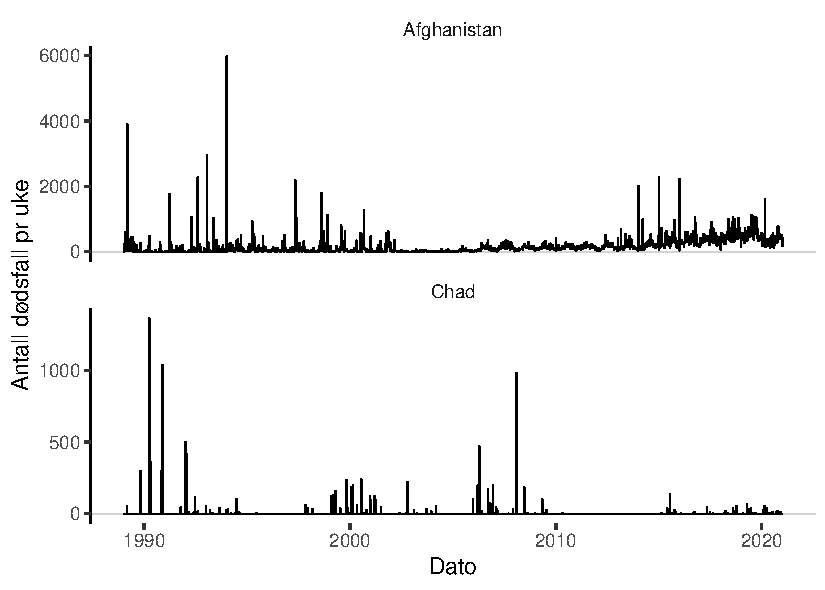
\includegraphics{../img/weekly_deaths}
    \caption{Ukentlig antall drepte i konflikter der staten er en aktør i
        Afghanistan og Chad. Gjennomsnittet er markert med rød linje.}
    \label{fig:weekly_deaths}
    \end{figure}

Samtidig som disse dataene gir nye muligheter for prediksjon og inferens, er
det også utfordringer knyttet til modelleringen av UCDP-dataene. I
\cref{fig:weekly_deaths} kan man se eksempler på ukentlig dødsfall for to
forskjellige land, ett med mange dødsfall pr uke (Afghanistan) og ett hvor det
er lengre tidsintervall mellom uker med dødsfall (Chad). Figuren illustrerer
noen av utfordringene som følger med når man skal modellere på slike data.
For et land som Chad er det overvekt av uker hvor det er 0 dødsfall, såkalt
zero-inflation. Det andre som kommer frem er at variansen er mye høyere enn
forventningen, såkalt overspredning. Videre er responsvariabelen diskret og
nedad begrenset til 0. En sannsynlighetsfordeling som tar høyde for både
zero-inflation og overspredning er nødvendig for å modellere dataene.

I denne oppgaven vil vi se på to mulige modeller for å predikere antall
dødsfall en uke fram i tid i konflikter mellom en statlig og ikke statlig
aktør. Vi vil sammenligne en modell som antar at logaritmen til antall dødsfall
er normalfordelt med en modell hvor vi antar at antall dødsfall er
negativ-binomialfordelt. Vi vil forsøke å vurdere modellene med tanke på hvor
gode de er til å estimere antall dødsfall en uke fram i tid og se hvor gode de
prediktive distribusjonene beskriver de observerte dataene.
 



\section{Data}

\textit{Uppsala Conflict Data program} samler inn og verifiserer data om
konflikter og organisert vold i hele verden. Et av datasettene,
\textit{Georeferenced Event Dataset (GED)} består av dødsfall som et resultat
av organisert vold. Organisert vold er i denne sammenhengen hendelser i en
konflikt som har resultert i dødsfall, og hvor minst en part i konflikten er en
organisert enhet. Hvert datapunkt i GED er definert som en hendelse. For at en
hendelse skal bli inkludert i datasettet må det ha skjedd minst et verifisert
dødsfall. Dataene blir samlet inn fra nyhetskilder, rapporter fra forskjellige
autoriteter og organisasjoner, og blir forsøkt verifisert fra flere kilder.
Tidspunkt og sted for hendelsene blir estimert med størst mulig nøyaktighet.
Informasjon om parter i konflikten blir også fastsatt. Datasettet starter med
hendelser fra 01.01.1989 og strekker seg fram til 31.12.2021. 


\begin{table}[!h]
\centering

\begin{tabular}[t]{llrrrrr}
\toprule
date\_start & country & date\_prec & type\_of\_violence & best & high & low\\
\midrule
2017-07-31 & Afghanistan & 1 & 1 & 6 & 6 & 6\\
2021-08-26 & Afghanistan & 1 & 1 & 183 & 184 & 171\\
2021-08-28 & Afghanistan & 1 & 1 & 2 & 3 & 0\\
$\vdots$ & $\vdots$ & $\vdots$ & $\vdots$ & $\vdots$ & $\vdots$ & $\vdots$ \\ 
 \bottomrule
\end{tabular}
\caption{De første radene i GED-datesettet. Variabler som ikke er relevante for
denne oppgaven er utelatt.}
\label{tab:GED_table}
\end{table}

Vi skal se på ukentlige antall dødsfall som resultat av organisert vold. Det
har vi definert som hendelser hvor staten er en aktør i konflikten. Hendelser i
konflikter mellom to ikke statlige aktører ble filtrert ut. Videre brukte vi
det beste estimatet for antall døde. Hendelser hvor tidspunktet ikke kunne
bestemmes mer nøyaktig enn på måned eller år, ble utelatt. Land med færre enn
100 uker med hendelser ble også utelatt. Antall dødsfall ble så aggregert for
hver uke i hvert land. For antall dødsfall pr hendelse bruker vi det beste
estimatet. I den endelige undersøkelsen endte vi opp med datasett med tre
variabler: uke, land og antall døde. Det vil si for hvert land har vi en
tidsserie med antall dødsfall pr uke mellom 01.01.1989 til 31.12.2021. Land med
færre enn 100 uker med hendelser ikke inkludert.

For å kvantifisere graden av overspredning av dødsfall for hvert land kan man
sammenligne den observerte fordelingen med en teoretisk poisson-fordeling med
samme forventning som de observerte dataene \parencite{weiss2018introduction}.
Dette gir opphav til  spredningsindeksen $I_{\mathrm{disp}}$. Gitt det
observerte gjennomsnittet $\hat{\mu}$ og den observerte variansen
$\hat{\sigma}^2$ blir 

 $$
    I_{\mathrm{disp}} = \frac{\hat{\sigma}^2}{\hat{\mu}}.
 $$

Ved $I_{\mathrm{disp}} = 1$ er variansen lik gjennomsnittet, noe som er
karakteristisk for poissonfordelingen. Er $I_{\mathrm{disp}} < 1$ har dataene
underspredning: I motsatt tilfelle når $I_{\mathrm{disp}} > 1$ har dataene
overspredning. 

Andelen 0-verdier ble brukt direkte som et mål for zero-inflation:

$$
\hat{p_0} = \frac{1}{N}\sum_{t=1}^N \mathds{1}(Y_{i,t}=0).
$$

    \begin{figure}[!h]
    \centering
    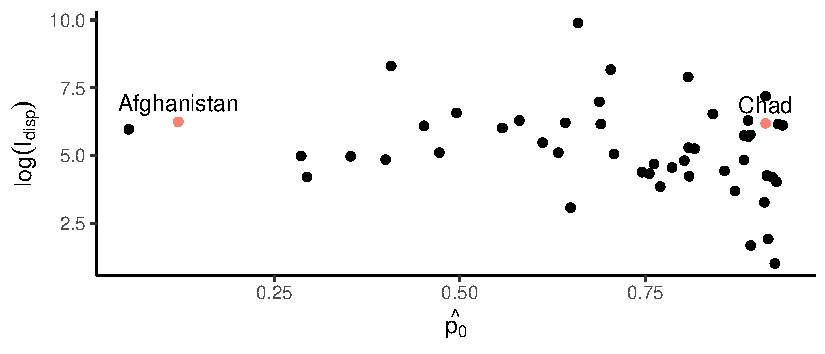
\includegraphics{../img/index_plot.pdf}
        \caption{
            Logaritmen til $I_{\mathrm{disp}}$ og andel 0-verdier ($\hat{p_0}$) for
            de inkluderte landene. Chad og Afghanistan er uthevet.
        }
    \label{fig:index_plot}
    \end{figure}

I \cref{fig:index_plot} vises en oppsummering av spredningsindeksen og andelen
0-verdier for alle landene som er inkludert. Afghanistan og Chad har omtrent
samme spredningsindeks, men er i hver ende av skalaen for andelen 0-verdier.



\section{Modellering}

Vi har valgt å sammenligne negativ-binomialfordelingen og lognormalfordelingen
som grunnlag estimere antall dødsfall en uke fram i tid. Vi vil ta utgangspunkt
i en tidseriemodell som estimerer antall dødsfall i uke $t$ ut fra antall
dødsfall i uke $t-1$. 

En modell som er sentral i tidsserieanalyse er den autoregressive modellen (AR).
Modellen legger til grunn at det finnes korrelasjon mellom observasjonene i
en tidsserie. Ved å bruke korrelasjonen kan man prøve å estimere
sannsynligheten for fremtidige utfall av verdier i tidsserien. Antall verdier
fra tidsserien man inkluderer avgjør hvilken orden modellen har. I dette
tilfellet bruker vi observasjonene fra forrige tidssteg $t-1$ i modellen, så
det blir en 1. ordens autoregressiv modell (AR(1)). En standard AR(1)-modell
for kontinuerlig responsvariabel er formulert ved  

$$
Y_t|Y_{t-1} = a + bY_{t-1} + \epsilon_t,
$$

\noindent
der $a \in \mathbb{R}$, $0 < |b| <1$, og $\epsilon_t$ er feilen ved uke $t$.
Vider antar man at $\epsilon_t$ er en tilfeldig variable som er normalfordelt
med forventning 0 og standardavvik $\sigma$. For at AR(1)-modellen skal være
stasjonær kreves det at $b$-parameteren er begrenset til $|b| < 1$. At modellen
er stasjonær betyr at det finnes en marginal sannsynlighetsfordeling over $Y$
når $t \to \infty$. Hvis $|b| > 1$ vil modellen beskrive en tidsserie som er
ustabil og som kan vokse ubegrenset. 

Siden vi skal beskrive dødsfall, som er ikke negative heltall er det nødvendig
å gjøre noen modifikasjoner for å kunne bruke en AR(1)-modell. Det ene man kan
gjøre er å transformere responsvariabelen slik at den er representert som et
rasjonelt tall, vanligvis er det gjort ved å ta logaritmen til variabelen. En
annen metode er å finne forventningen betinget på observasjoner ved $t-1$ og så
finne en heltallsfordeling som beskriver observasjonene ved tid $t$ gitt
observasjonene ved tid $t-1$ \parencite[73]{weiss2018introduction}. For vårt eksempel vil den betingede forventningen
være 

$$
M_t|Y_{t-1} = a +bY_{t-1}.
$$

\noindent
Så lar man $Y_t ~ F(M_t)$ der $F$ er en heltallsfordeling. Hvis $F$ er
Poisson-fordelingen blir  

$$
Y_t|Y_{t-1} \sim \mathrm{Poi}(M_t|Y_{t-1}).
$$

\noindent



\subsection{Negativ binomial}

Den første modellen vi skal se på er en modell tilpasset heltallstidsserier med
overspredning. Modellen er beskrevet av \cite{xu2012model} og er en Negative
Binomial Dispersed Integer Auto Regressive Conditional Heteroscedasity-modell
(NB-DINARCH). Modellene blir referert til som NB-modellen i resten av oppgaven.
Ved å bruke negativ-binomialfordelingen har man mulighet til å modellere data
med overvekt av 0-verdier og overspredning. Dette er i motsetning til en modell
basert på Poisonnfordelingen, hvor den betingede variansen er lik den betingede
forventningen. La $Y_{i, t} \in \mathbb{N}_0$ være antall dødsfall i land $i$ i
uke $t$. Videre er den betingede forventningen

$$
M_{i, t}|Y_{i,t} = a_i + b_iY_{i,t-1},
$$

\noindent
hvor $a > 0$ og $0 < b < 1$. Da er modellen definert av

$$
Y_{i,t}|Y_{i, t-1} \sim 
\mathrm{NB}\left(c(M_{i,t}|Y_{i, t-1}), \frac{c}{c+1}\right),
$$

\noindent
hvor $c >0$. Forventningen til $Y_{i,t}|Y_{i,t-1}$ blir

$$
\mathrm{E}[Y_{i,t}|Y_{i,t-1}] = a + bY_{i,t-1}.
$$

\noindent
Variansen blir

$$
\mathrm{Var}(Y_{i,t}|Y_{i,t-1}) = \frac{(a + bY_{i,t-1})(c + 1)}{c}.
$$

\noindent
Parameteren $a$ blir en grunnrate i antall dødsfall pr uke. Parameteren $b$ er
en skaleringsfaktor som sier noe om hvor sterk sammenheng det er mellom dødsfall
i en uke til den neste. Parameteren $c$ påvirker spredningen til fordelingen.
Her ser man at forventningen er uavhengig spredningsparameteren $c$. Derimot
varierer variasjonen med forventningen. Dette gjør at modellen kan beskrive
populasjoner med både høye og lave forventninger. Vi kan og så se at variansen
går mot forventningen når $c \to \infty$, det vil si en Poisson-fordeling med
forventning og varians $M_{i,t}$. Modellen er dermed egnet til å beskrive
populasjoner med overspredning, da variansen kan anta verdier fra $M_{i,t}$
til $\infty$.

\subsection{Lognormal}

Den andre fordelingen vi skal bruke er lognormalfordelingen. Motivasjonen for å
bruke denne fordelingen i modelleringen er at man får redusert
heteroskedasiteten når verdiene er på den logaritmiske skalaen. En annen grunn
til å operere på logaritmisk skala er at modelleringen kan bli enklere. En anne
grunn er at ikke negative heltall er transformert til å være rasjonale tall. Da
kan modelleringen bli enklere og man kan bruke for eksempel en standard
AR(1)-modell.

Hvis $Y_{i,t}$ er antall dødsfall i land $i$ i uke $t$ definer vi den transformerte variabelen

$$
Z_{i,t} = \log(Y_{i,t} + 1).
$$
\noindent
Vi tar logaritmen av $Y_{i,t} + 1$ for at omgå at man tar $\log(0)$. Videre antar vi da at

$$
Z_{i,t}|Z_{i,t-1} = a_i + b_iZ_{i,t-1} + \epsilon_{i,t},
$$

\noindent
der $\epsilon_{i,t} \sim \mathrm{N}(0, \sigma_i)$.  Her er $a_i > 0$, $0 < b_i
< 1$ og $\sigma_i > 0$. Parameteren $a_i$ grunnraten til $Z_{i,t}$. Parameteren
$b_i$ er beskriver sammenhengen mellom $Z_{i, t-1}$ og $Z_{i,t}$. Parameteren
$\sigma_i$ beskriver standardavviket til $\epsilon_{i, t}$. Forventningen til
$Z_{i,t}|Z_{i,t-1}$ er

$$
Z_{i,t}|Z_{i,t-1} = a_i + b_iZ_{t-1}
$$

\noindent
og variansen er $\sigma_{i}^2$. Videre er forventningen til $Y_{i,t}|Z_{i,t-1}$

$$
\mathrm{E}[Y_{i,t}|Z_{i,t-1}] = e^{a_i +b_iZ_{t-1} \frac{\sigma_i^2}{2}} - 1.
$$

Variansen til $Y_{i,t}|Z_{i,t-1}$ er

$$
\mathrm{Var}(Y_t|Z_{i,t-1}) = (e^{\sigma_i^2}-1)e^{2(a_i+b_iZ_{i,t-1}) + \sigma_i^2}.
$$

En detalj å legge merke til  er at $\mathrm{E}[Y_{i,t}|Y_{i,t-1}]$ er avhengig
av spredningsparameteren $\sigma$. Selv om man på lognormalskalaen kan
modellere data med lav forventning og høy varians, vil forventningen på
originalskalaen øke med variansen. 



\section{Estimering}

Med denne undersøkelsen ønsket vi å undersøke hvordan de betingede
prediksjonsfordelingene oppfører seg. Derfor ble parametrene i modellene
estimert med hele tidserien. Vi estimerte parametrene for hvert land til de to
modellene med betinget maksimum likelihood (CML). For negativ binomialmodellen
ble parametrene ble valgt slik at funksjonen

$$
\ell_{n_i}(a_i, b_i , c_i| Y_{i, 1}) = \sum_{t=2}^{n_i} \log(f(Y_{i,t}|a_i, b_i, c_i, Y_{i, t-1}))
$$

\noindent
ble minimert. Funksjonen $f(\cdot)$ er 

$$
\mathrm{P}(Y=Y_{i,t}|a_i, b_i, c_i, Y_{i, t-1}),
$$

\noindent
der $\mathrm{P}$ er gitt ved den betingede negativ binomialtetthetsfunksjonen.
For lognormalmodellen ble funksjonen

$$
\ell_{n_i}(a_i, b_i , \sigma_i| Y_{i, 1}) = \sum_{t=2}^{n_i} \log(g(Y_{i,t}|a_i, b_i, \sigma_i, Y_{i, t-1}))
$$

\noindent
minimert. Her er $g(\cdot)$ den negative logaritmen til tetthetsfunkjonen til
normalfordelingen. Funksjonene ble minimert numerisk ved hjelp av
\texttt{optim} funksjonen i R. For å sikre stabile estimater ble funskjonen
kjørt 10 ganger, og paramtrene som ga lavest loglik-verdier ble valgt.


\section{Evaluering og diagnostisering}

Hvor god en modell er avhenger av hvilket formål modellen skal brukes til. Skal
modellen brukes til å komme med en punktprediksjon kan det være at man ønsker
at modellen skal ha lav absolutt feil. I andre tilfeller er man interessert i at
modellen skal gjenspeile spredningen i observasjonene. Vel så viktig kan det
være å estimere sannsynligheten for at det kommer en eller flere hendelser i
neste uke, $P(Y_{i, t+1} > 0)$, som det er å prøve å estimere den faktiske
størrelsen. For å komme med estimater på sannsynligheter for intervaller av
verdier er det nødvendig at den prediktive fordelingen passer til de observerte
dataene. Hvor godt modellen beskriver dataene kalles kalibrering. Hvor godt
modellen er kalibrert kan bedømmes gjennom diagnostiske plot. Hvor konsentrert
modellen er rundt punktestimatet kalles for skarphet. Skarphet kan bedømmes
gjennom \textit{scoring rules} \parencite{czado2009predictive}. 


\subsection{Kvadrert feil}

For å se på hvor godt modellene gjør punktprediksjoner er den kvadrerte feilen
(RMSE) av interesse.  Det er viktig å være oppmerksom på at prediksjonene her
gjøres på de samme dataene som er brukt til å estimere parametrene i modellene,
og man kan få overtilpassede modeller hvis man bare ser på RMSE.  

$$
\mathrm{RMSE}=\sqrt{\frac{1}{n}\sum_{i=1}^n(\hat{y}_i-y_i)^2}
$$

RMSE sier imidlertid ingenting om variansen. For å se på feilen relativ til
hvor stor spredning modellen estimerer kan man normalisere feilen ved å dele på
variansen (RMNSE). Også ved bruk RMNSE som et mål på hvor godt modellene gjør
må man være varsom. En modell som overestimerer variansen vil ha lavere RMNSE
sammenlignet med en modell med samme forventning, men lavere varians.

$$
\mathrm{RMNSE}=\sqrt{\frac{1}{n}\sum_{i=1}^n \left(\frac{\hat{y}_i-y_i}{\hat{\sigma}_i}\right)^2}
$$

\subsection{Scoring rules}

En scoring rule er en oppsummering av modellen og observasjonene i form av et
tall. Når man sammenligner modeller svarer et lavere tall til en modell som
beskriver dataene bedre. Fra \citep{czado2009predictive} er en scoring rule er
proper hvis for en fordeling $Q$ en fordeling $P$ og en scoring rule $s$ har
følgende forhold:

\begin{equation}
s(Q, Q) \leq s(P, Q)
    \label{eq:proper}
\end{equation}

Her er $Q$ fordelingen som etter modellererens dømme er den sanne fordelingen
av dataene. Hvis (\ref{eq:proper}) har likhet kun hvis $P = Q$ er $s$ strikt
proper. Strikt propre scoring rules gir et mål på både kalibrering og skarphet. 

En proper scoring rule er Dawid-Sebastini score
\parencite{gneiting2007strictly}. Den inkorporerer variansen og standardisert
feil samtidig. 


$$
\mathrm{DS}(P, x) =\frac{1}{n}\sum_{i=1}^n \left(\frac{\hat{y}_i - y_i}{\hat{\sigma}_i}\right)^2 + 2 \log \hat{\sigma}_i.
$$

I DS-scoren øker det andre leddet når variansen øker. Motsatt øker det første
leddet hvis variansen synker. En annen scoring rule som både tar hensyn til
punkt-prediksjonen og prediksjonsintervallet er \textit{Ranked Probability
Score (RPS)}. RPS til en observasjon $x$ kan skrives som 

$$
RPS(P_i,x) = \frac{1}{n}\sum_{i=1}^n \mathrm{E}|X - y_i| - \frac{1}{2}\mathrm{E}|X - X'|,
$$

\noindent
der $P_i$ er en betinget sannsynlighetsfordeling. $X$ og $X'$ er to uavhengige
variabler fra fordelingen $P_i$ \parencite{gneiting2007strictly}. Har $P_i$
stor spredning vil både første og andre ledd øke. Samtidig vil en $P_i$ som
legger mye vekt rundt $y_i$ gi lave verdier i det første leddet.

\subsection{PIT-diagram}

En annen måte å diagnostisere modellene på er å plotte de predikerte kvantilene
i den observerte fordelingen mot kvantilene i den prediktive fordelingen. I
\citep{czado2009predictive} anbefales det å plotte et Probability Integral
Transform (PIT) diagram for å undersøke om den prediktive distribusjonen
beskriver de observerte dataene. For diskrete data foreslår
\citep{czado2009predictive} følgende måte å regne ut PIT-score for et utvalg.
For en verdi $u \in [0, 1]$ og en observasjon $y$ regner man først ut 

$$
F(u|y) = \begin{cases}
    0, & \quad u < P_{y-1} \\
    \frac{u - P_{y-1}}{P_y - P_{y-1}}, & \quad P_{y-1} \leq u \leq P_y \\
    1, & \quad P_y < u
         \end{cases}  
.
$$

Her er $P$ den kumulative tetthetsfunksjonen for $y_t | y_{t-1}$. For å
diagnostiserer modellen kan man se på $\overline{F}(u) =
\frac{1}{n}\sum_{i=1}^nF(u|y_i)$. Hvis $y \sim P$ så vil $\overline{F}(u)$ gå
mot $u$ når $n \to \infty$. Nå kan man plotte $\overline{F}(u)$ mot $u$, eller
så kan man definere en ny variabel:

$$
F(j)= \overline{F}\left(\frac{j}{J}\right) 
- \overline{F}\left(\frac{j-1}{J}\right),
$$

\
der $j \in \{1\,2,\ldots,J \}$ for en valgt verdi av $J$. Lager man et
histogram der søylene har høyde $F(j)$ vil strukturen på histogrammet gi
informasjon om hvordan de observerte verdiene forholder seg til
prediksjonsfordelingen. Hvis observasjonene $y \sim P$ vil søylene være nær
like høye for alle $j$. Et histogram med form som en u snudd opp ned indikerer
at den observerte fordelingen er tettere enn det som er forventet under den
estimerte fordelingen. Motsatt vil et u-formet histogram indikere at modellen
forventer lavere spredning en det som er observert. I \cref{fig:pit_explain}
ser man et eksempel med simulerte data. PIT-histogrammer for 200 verdier
trukket fra en negativ binomialfordeling med parametere $r=5$ og $p=0.5$. 

    \begin{figure}[!h]
    \centering
    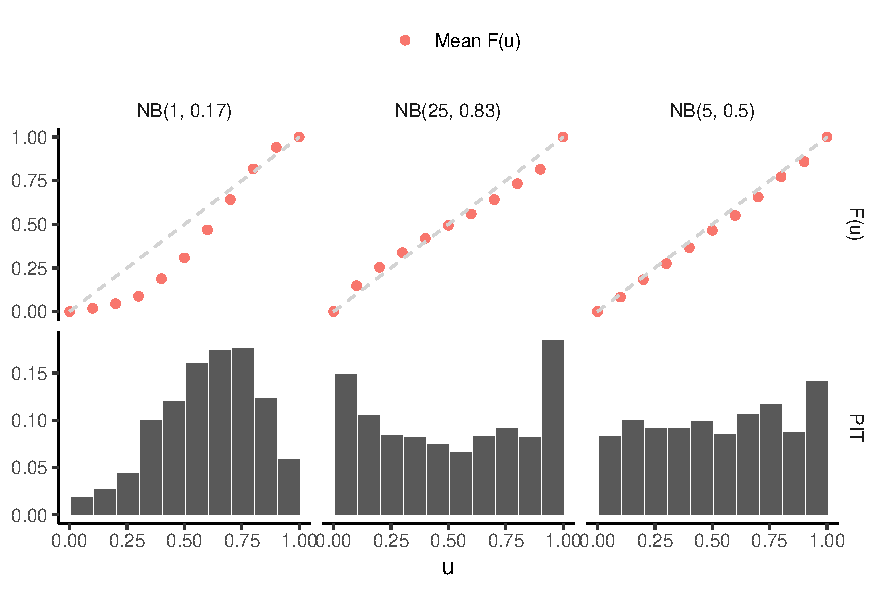
\includegraphics{../img/pit_explain.pdf}
    \caption{
        $F(u)$ og PIT-diagram for 200 tilfeldige verdier trukket fra en
        $\mathrm{NB}(5, 0.5)$-fordeling, med forventning 5 og varians 10.
        $F(u)$ og PIT-diagrammet er regnet ut fra 3 fordelinger med forventning
        5, men med forskjellig varians. I den første raden ses
        $\overline{F}(u)$, den nederste raden viser PIT-diagrammet. I den
        første kolonnen er en modell med overspredning (varians 150). Den andre
        kolonnen viser $F(u)$ og PIT-diagram for en modell med underspredning
        (varians $\frac{6}{5}$) Den siste kolonnen viser $F(u)$ og PIT-diagram
        regnet ut fra originalfordelingen. Eksemplet er adaptert fra
        \cite{czado2009predictive}
    }
        \label{fig:pit_explain}
    \end{figure}



\clearpage
\section{Resultater}

Vi skal nå se nærmere på Chad og Afghanistan som eksempler på land med
forskjellige antall og frekvens av hendelser. Chad er et land med mye 0-verdier
(høy $\hat{p_0}$). Afghanistan er i den andre enden av skalene med lav andel
0-verdier (lav $\hat{p_0}$). Begge landene viser overspredning i antall
dødsfall.. Videre vil vi vurdere modellene når man ser på alle landene under ett.
Vi har også sammenlignet modellene med en variant av en 0-modell, $Y_t|Y_{t-1}
= Y_{t-1}$. Det vil si en modell som predikerer at antall dødsfall i neste uke
er det samme som antall dødsfall i denne uken, en såkalt no change-modell (NC).

Sammenhengen mellom prediksjonener og observasjonene kan man se på
residualene. I \cref{fig:residuals_orig} er de ustandardiserte residualene
plottet for Chad og Afghanistan. Modellene overestimerer ved lave observerte
dødsfall og underestimerer ved høye observerte dødsfall. De standardiserte
residualene viser bedre hvordan de to fordelingene skiller seg fra hverandre
(\cref{fig:residuals}). For Afghanistan predikerer begge modellene ganske likt,
men LN-modellen underestimerer i større grad for de ekstreme verdiene. For Chad
har NB-modellen noe lavere standardiserte residualer en LN-modellen.  

Residualene alen er ikke nok for å bedømme modellene. I
\cref{tab:scoring_summary} vises den kvadrerte feilen og scoring rules. For
alle land sett under ett har LN-modellen lavest feil, det vil si prediksjoner
som er nærmest de observerte verdiene. For de normaliserte feilene er NB og
NC-modellene de som har lavest feil. For DSS og RPS ser man også at NB-modellen
gjør det bedre enn LN-modellen. No-change modellen sett over alle land lavest DSS-score.  

\begin{figure}[!h]
\centering
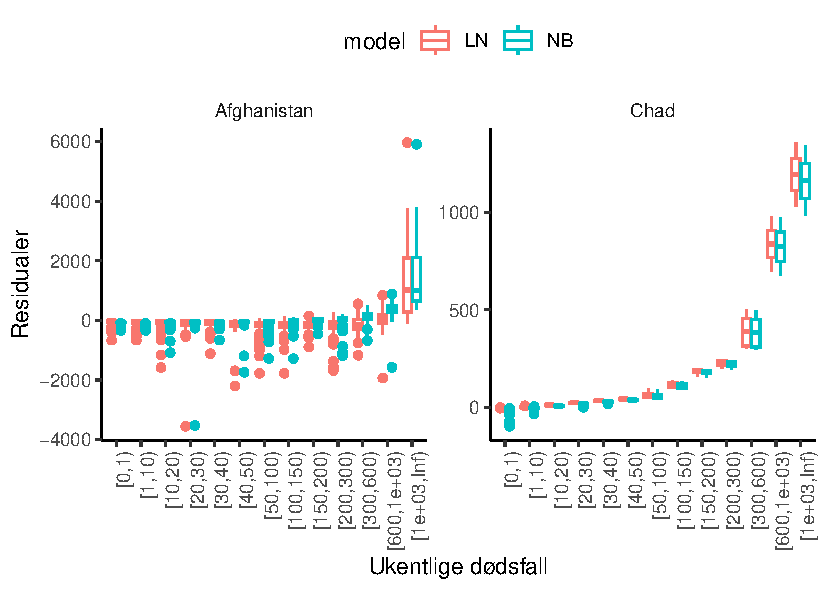
\includegraphics{../img/res_orig.pdf}
\caption{
    Antall dødsfall og residualer for Chad og Afghanistan.
    } 
\label{fig:residuals_orig}
\end{figure}

\begin{figure}[!h]
\centering
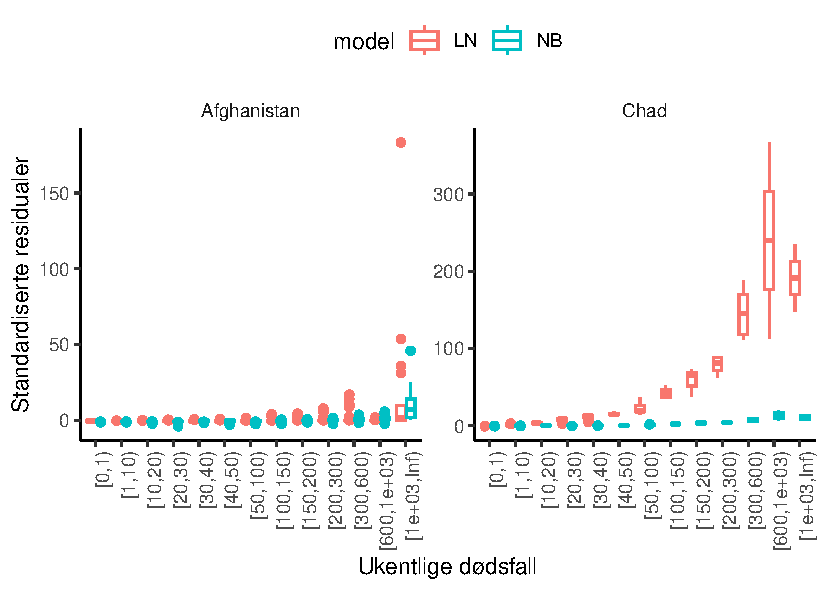
\includegraphics{../img/residuals.pdf}
\caption{Standardisert antall dødsfall og standardiserte residualer for Chad og
    Afghanistan. Antall dødsfall er standardisert ved å dele på variansen for
    landet.} 
\label{fig:residuals}
\end{figure}

I \cref{fig:pred_plot} vises prediksjonsintervallet for de prediktive
fordelingene gitt antallet dødsfall ved $t-1$. For Afghanistan har NB-modellen
et smalere intervall enn LN-modellen. For Chad har LN-modellen brutt sammen og
har mest vekt ved verdier nærme 0. LN-modellen ignorerer variasjonen i
observasjonene.  

\begin{figure}[!h]
\centering
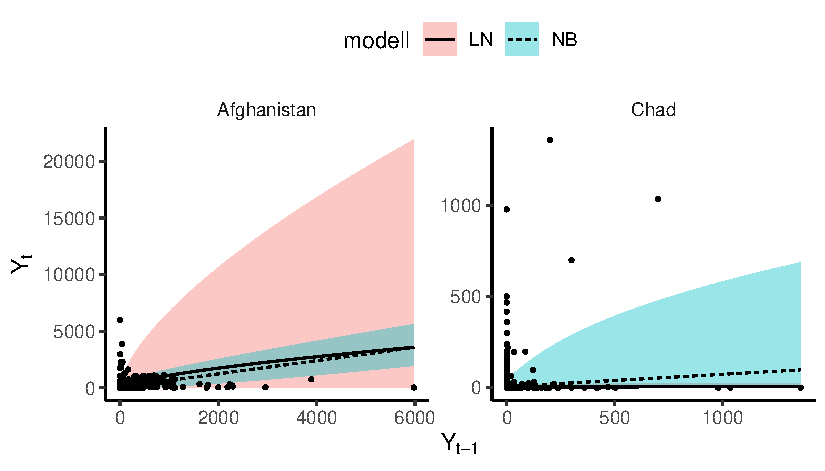
\includegraphics{../img/pred_plot.pdf}
\caption{
    Antall dødsfall ved $t-1$ mot antall dødsfall ved tid $t$. Et 95 \%
    prediksjonsintervall for hver av modellene er markert med henholdsvis rødt
    (LN) og grønt (NB). Forventningen er markert med hel linje (LN) og stiplet
    linje (NB). LN-modellen er så vidt synlig som et smalt bånd nederst.
} 
\label{fig:pred_plot}
\end{figure}

\begin{table}[!h]
\centering

\begin{tabular}[t]{llrrrr}
\toprule
Land & Modell & RMSE & RMNSE & DSS & RPS\\
\midrule
Afghanistan & LN & 178.39 & 0.54 & 36.18 & 94.56\\
Afghanistan & NB & 120.26 & 0.62 & 13.64 & 89.37\\
Afghanistan & NC & 120.23 & 0.34 & 12.76 & -\\
\addlinespace
Alle land & LN & 18.03 & 1.30 & 360.36 & 14.61\\
Alle land & NB & 19.38 & 0.40 & 10.51 & 14.14\\
Alle land & NC & 20.48 & 0.20 & 8.54 & -\\
\addlinespace
Chad & LN & 8.13 & 2.55 & 261.33 & 7.42\\
Chad & NB & 13.00 & 0.22 & 8.78 & 6.99\\
Chad & NC & 12.42 & 0.17 & 9.63 & -\\
\bottomrule
\end{tabular}
    \caption{Tabell over skåringsverdiene, RMSE og standardiserte RMSE
    (RMNSE), samt Dawid-Sebastini score (DSS) og Ranked Probability Score
    (RPS).}
\label{tab:scoring_summary}
\end{table}

\begin{figure}[!h]
\centering
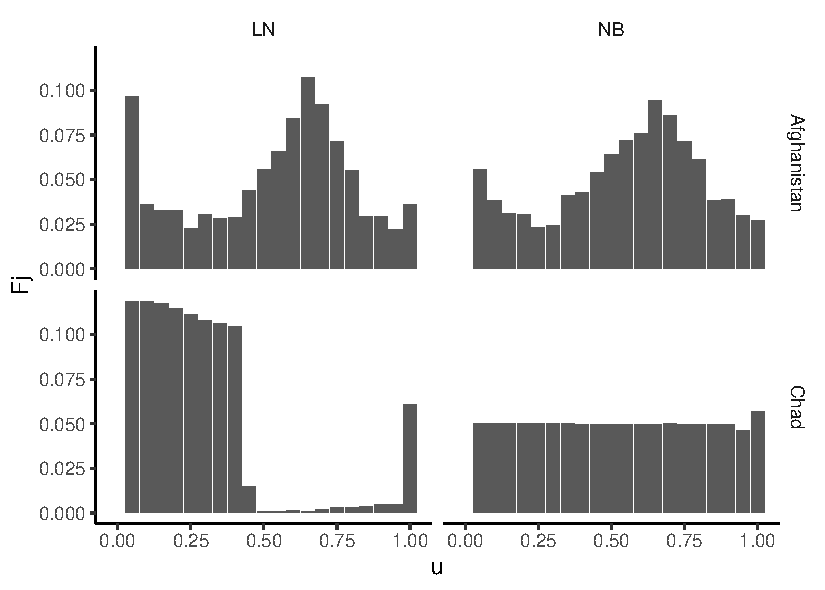
\includegraphics{../img/PIT_plot.pdf}
\caption{
    PIT-diagram for begge modellene for Afghanistan og
    Chad. 
}
\label{fig:PIT_plot}
\end{figure}

PIT-plottet (\cref{fig:PIT_plot}) viser at for Afghanistan er det overspredning
i de prediktive fordelingene. De høye søylene i PIT-plottet lognormal-modellen
i Afghanistan (øverste panel til venstre) er det antydninger til at det er noen
ekstremverdier som er større enn forventet ut fra modellen. For Chad er
forskjellen mellom modellene tydelige. Negativ binomialmodellen viser et flatt
histogram, noe indikerer fordelingen tilnærmer seg de observerte verdiene i
stor grad. Lognormal-modellen derimot har en prediktiv fordeling som tydelig har underspredning.  

For å si noen hvor de to modellene gjør det bra og hvor de bryter sammen har vi
plottet andelen 0-verdier mot feilen og DSS-score (\cref{fig:p0_plot}). For
RMSE ser vi at ved en andel 0-verdier over 0.7 er den RMSE lav. Den
standardiserte feilen RMNES er jevnt over lavere for NB-modellen jo høyere
andel 0-vedier. LN-modellen har større RMNES dess høyere andel 0-verdier. Det
samme mønsteret viser seg på DSS-score, med noen unntak hvor LN-modellen har
lavere score. Dette understøtter at LN-modellen legger mer vekt på 0-verdiene
verdiene på bekostning av å estimere variasjonen.


Videre har vi plotte spredningsindeksen $I_{\mathrm{disp}}$ mot RMSE, RMNSE og
DSS-score (\cref{fig:disp_plot}). RMSE øker for begge modellene når
$I_{\mathrm{disp}}$ øker. RMNSE øker for LN-modellen, men ikke for NB-modellen.
For begge modellene øker DSS-scoren med $I_{\mathrm{disp}}$, men mer for
LN-modellen.

\begin{figure}[!h]
\centering
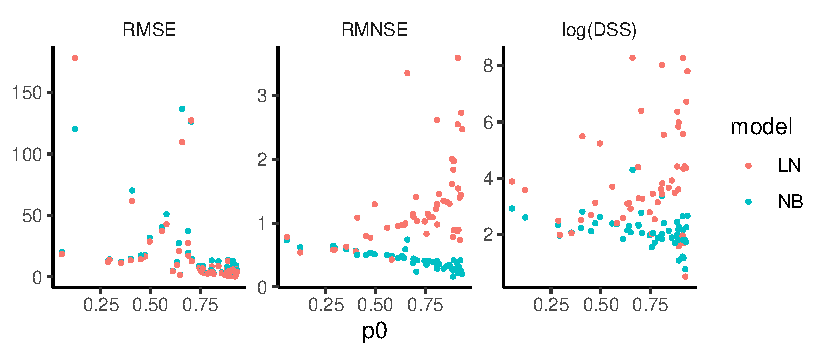
\includegraphics{../img/p0_plot.pdf}
\caption{
    Andelen 0-verdier plottet mot RMSE, normalisert RMNSE og log(DSS) for alle
    land for de to modellene.
}
\label{fig:p0_plot}
\end{figure}

\begin{figure}[!h]
\centering
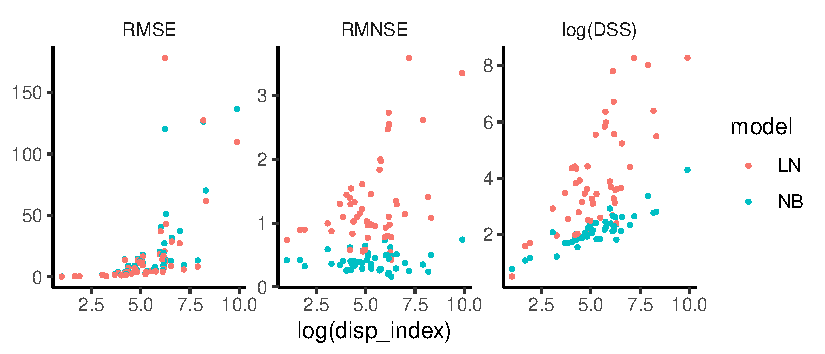
\includegraphics{../img/disp_plot.pdf}
\caption{
    Spredningsindeksen plottet mot RMSE, normalisert RMNSE og log(DSS) for alle
    land for de to modellene.
}
\label{fig:disp_plot}
\end{figure}



\clearpage
\section{Konklusjon}

Som vi har vist har lognormal-modellen bedre punktprediksjon enn NB-modellen,
men det kan like gjerne være  overvekt av 0-verdier som gjør punktprediksjonene
bedre. Som nevnt tidligere vil en modell som predikerer verdier rundt 0 ha lav
feil når mesteparten av verdiene er 0 verdier. Her blir det en byttehandel hvor
man får bedre punktprediksjoner, men hvor man har introdusert en skjevhet på
estimatene av modell-parametrene. Dette ser man i PIT-diagrammet i
\cref{fig:PIT_plot}. Vi ser muligens at modellens betingede prediktive
fordelinger ikke egner seg til å beskrive de observerte verdiene. Den
prediktive fordelingen kan bli veldig smal. Dette ser man særlig når andelen 0
verdier er høye (se \cref{fig:pred_plot}, Chad). At lognormal-modellen får
problemer med høye 0-verdier understøttes også at den får høyere DSS-score og
standardisert feil når andelen 0-verdier øker (\cref{fig:p0_plot}). 

NB-modellen er man er bedre kalibrert enn lognormal-modellen. Dette går fram
fra PIT-plottet i \cref{fig:PIT_plot}. Selv om punktprediksjonen er dårligere,
er NB-modellen bedre til å estimere den betingede prediksjonsfordelingen. Dette
trenger vi for å få svar på spørsmål som "hva er sannsynligheten for at det
forekommer tap av menneskeliv i neste uke ($\mathrm{P(Y_{i,t+1} > 0|
Y_{i,t})}$)?". 

I denne undersøkelsen har vi brukt en relativt enkel modell som kun betinger på
antall dødsfall ved uke $t-1$. Begge modellene får problemer med å takle
overgang fra ingen dødsfall en uke til mange den neste uken. Hvis andel
0-verdier er høy vil en No-change modell typisk ha lav feil. Videre er
parametrene estimert ut fra hele tidsserien, noe som tilsvarer en antagelse om
at parametrene ikke endrer gjennom den observerte perioden. Det er mulig at
modellene hadde gjort det bedre ved å legge større vekt på observasjoner som
er nærmere i tid. Man kan tenke seg at man estimerer parametrene kun på
observasjoner fra en måned, et halvår eller år tilbake.

Disse enkle modellene gir gir grunnlag for å utforske negativ
binomial-fordelingen og lognormal-fordelingen videre. En retning som kunne være
av interesse er å tilpasse AR-modeller av høyere orden. Dette er modeller
som ikke bare betinger på den foregående uken, men kan betinge på flere uker i
forkant. En annen retning som kan være av interesse er å sammenligne de to
fordelingene oppfører seg når prediksjonen går over korter eller lengre
tidsintervall. I \cref{fig:monthly_res_plot} vises de standardiserte
residualene for de samme modellene, men hvor ukentlige dødsfall er byttet ut
med månedlige dødsfall. Her ser man spesielt for Chad at det er mindre
forskjell mellom modellene enn når man ser på ukentlige data
(\cref{fig:residuals_orig}).

\begin{figure}[!h]
\centering
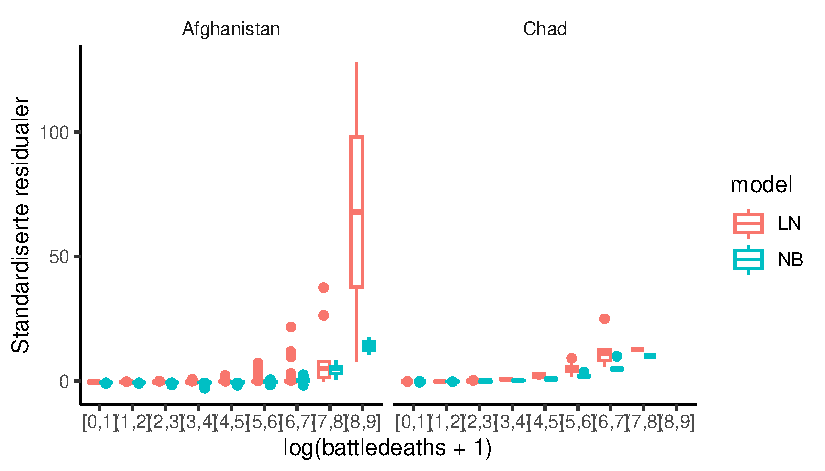
\includegraphics{../img/monthly_res_plot.pdf}
\caption{
    Månedlige log(dødsfall + 1) og standardiserte residualer for Afghanistan og
    Chad.
} 
\label{fig:monthly_res_plot}
\end{figure}


Vi har vist at lognormalfordelingen kan brukes til å få et punktestimat av
antall dødsfall, selv om den prediktive fordelingen ikke beskriver de
observerte dataene. Vi har også vist at negativ binomialfordelingen er mer
fleksibel når man skal modellere data med overspredning og overvekt av
0-verdier.  Vi har og vist at data med stor andel 0-verdier er utfordrende å
modellere. Tidsseriemodellene får problemer når andelene 0-verdier er store.
Når det gjelder punktestimat er vanskelig å utkonkurrere veldig enkel modeller
som NC-modellen (No Change). Det kan være interessant å utforske hvordan de to
fordelingen oppfører seg når perioden man ønsker å predikere for er enten
større eller mindre enn en uke. Videre kan man undersøke hvordan fordelingene
oppfører seg når de brukes sammen med modeller som betinger på flere variabler







\clearpage

\printbibliography{}

\section*{Vedlegg}

All kode for databehandling, generere figurer og tabeller kan lastes ned fra 
\url{https://github.com/kongpottifar/STK_MAT_2011_prosjekt}

\end{document}
